\documentclass[]{article}

% to define bibliography and insert cites
\usepackage[backend=biber]{biblatex}
\addbibresource{references.bib}

% to insert framets of code
\usepackage{listings}

% to make links clickable
\usepackage{hyperref}
\hypersetup{colorlinks=false,linktoc=all}

% include images
\usepackage{graphicx}
\usepackage{float}

%opening
\title{Sistema de detección automática de socavones en el asfalto a partir de imágenes}
\author{Diego Castro Viadero}
\date{Septiembre 2019}

\renewcommand*\contentsname{Contenido}
\renewcommand{\figurename}{Figura}

\begin{document}

\maketitle

\begin{poliabstract}{Resumen}
\noindent
El estado del asfalto en carreteras tanto de ámbito nacional como de ámbito urbano es de alta importancia en relación a la seguridad vial. En la actualidad, gracias a los avances tecnológicos, se están desarrollando sistemas de detección automática de baches en el asfalto, permitiendo una detección precoz de estas irregularidades en la carretera.

\doublespacing\singlespacing
\noindent
Este proyecto pretende contribuir en este ámbito desarrollando un sistema de detección automática de baches a partir de imágenes. Partiendo de un conjunto de imágenes etiquetadas con baches, se ha entrenado una red neuronal \textit{YOLO V3} y otra \textit{YOLO V3 Tiny}. El entrenamiento se ha realizado con distintos tamaños de red y con distintos subconjuntos de imágenes, dando lugar a un total de quince modelos. Tras un estudio comparativo de las precisiones de los modelos, aquellos con mejores resultados han sido exportados y transformados para ser ejecutables en un dispositivo móvil. Finalmente se ha desarrollado una aplicación móvil Android que carga los modelos anteriormente exportados y los ejecuta utilizando como entrada la salida de la cámara del dispositivo.
\end{poliabstract}

\begin{poliabstract}{Abstract}
\noindent
The state of asphalt on both national and urban roads is of high importance in relation to road safety. Currently, thanks to technological advances, automatic detection systems are being developed to detect potholes in the asphalt, allowing early detection of these irregularities on the road.

\doublespacing\singlespacing
\noindent
This project aims to contribute to this field by developing an automatic pothole detection system based on images. Starting from a set of images labeled with potholes, a neural network YOLO v3 and another YOLO v3 Tiny have been trained. The training has been carried out with different network sizes and with different subsets of images, resulting in fifteen models. After a comparative study of the precisions of the models, those with better results have been exported and transformed to be executable in a mobile device. Finally, an Android mobile application has been developed that loads the previously exported models and executes them using the camera output of the device as input.
\end{poliabstract}

\newpage
\tableofcontents{}

\newpage
\section{Introducción}


% (2-4 páginas)

\subsection{Motivación y Objetivos}

% (porque has hecho este proyecto y que objetivos persigues)
% motivación: aplicar los conocimientos adquiridos durante el master en un proyecto "real"
% adquirir/complementar conocimientos que faltan en el máster

% objetivos: deseo de lo que se quiere

\textbf{!!! TODO}

\subsection{Estructura del trabajo}

% (este punto es pura formalidad. Se suele poner uno o dos párrafos explicando la estructura del proyecto como hacen en los libros)
% en el tema X se hablará de tatata, en el tema Y se hablará de blablabla

\textbf{!!! TODO} % (2-4 páginas)

\newpage
\section{Estado del arte}

% En el punto de motivación y objetivos debes de dejar muy claro que es lo que quieres hacer (un detector de baches) y en este tema 2 debes de explicar como se solucionan este tipo de problemas (CNN) y las redes y frameworks existentes para poder realizar tu trabajo. Como esto ya es una cosa que has hecho (me lo mandaste en un mail muy bien explicado) debes de contar los pros y contras y justificar el porque has seleccionado la red seleccionada % (como mucho 10 páginas)

\newpage
\section{Definición de requisitos y análisis}

% (2-4 páginas)

\subsection{Definición de requisitos}

% (que se quiere hacer definido de una manera formal)
% descripción del caso de uso

\textbf{!!! TODO}

\subsection{Arquitectura}

% (Haz un diagrama y luego explicalo, asi te valdrá para la presentación del proyecto)
% diagrama sencillo con la arquitectura: fotos + red neuronal + modelo + móvil

\textbf{!!! TODO}

\subsection{Tecnologías}

% (Esto es poco más que enumerar lo que vas a utilizar)
% python, keras, tensorflow, opencv, java, yolo v3, yolo v3 tiny

\textbf{!!! TODO} % (2-4 páginas)

\newpage
\section{Datos}

\subsection{Descripción de las fuentes de datos a utilizar}

El juego de datos ha sido obtenido de kaggle \cite{potholedataset} y se compone de un total de 1900 imágenes, tomadas desde el interior de un coche, con un tamaño igual a 3680x2760 píxeles (formato 4:3), y de un conjunto de ficheros de texto con el etiquetado de las mismas. Las imágenes se dividen en dos subconjuntos: uno de 1297 imágenes para el entrenamiento y otro de 603 imágenes para la evaluación del modelo. Por cada uno de los subconjuntos de imágenes existe un fichero de texto con el etiquetado de las mismas. Cada una de las líneas del los ficheros de texto contiene las etiquetas de una imagen. La estructura de cada línea es la siguiente:

\begin{lstlisting}[frame=single,basicstyle=\ttfamily\footnotesize]
<IMG_PATH> <NUMBER_OF_LABELS>( <X0> <Y0> <WIDTH> <HEIGHT>)+
\end{lstlisting}

Para facilitar el posterior tratamiento, se ha realizado una transformación del formato de los ficheros de etiquetas al siguiente formato:

\begin{lstlisting}[frame=single,basicstyle=\ttfamily\footnotesize]
<IMG_PATH>( <X0>,<Y0>,<WIDTH>,<HEIGHT>,<CLASS>)+
\end{lstlisting}

\subsection{Estudio de los datos}

En una fase inicial se ha realizado un análisis del tamaño de los socavones con respecto al tamaño de la imagen. Esto es un aspecto importante a tener en cuenta de cara a determinar el algoritmo a utilizar para la detección de objetos. Los algoritmos de detección de objetos, en general se comportan peor cuanto más pequeños son los objetos a detectar.

Como se observa en la figura \ref{fig:potholesizes}, la mayoría de los socavones tienen una anchura inferior a 200 píxeles y una altura inferior a 50 píxeles. Este factor será tenido en cuenta en el preprocesamiento de las imágenes.

\begin{figure}[H]
	\centering
	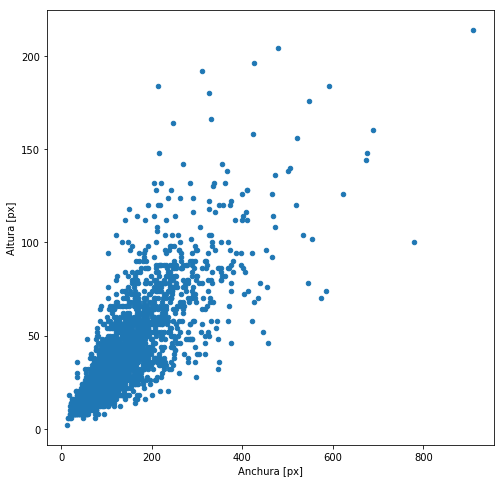
\includegraphics[width=0.8\linewidth]{images/pothole_sizes_scatter_plot.png}
	\caption{Tamaños de los socavones en píxeles}
	\label{fig:potholesizes}
\end{figure}

También se ha realizado un estudio de la localización de los socavones en las imágenes. Tal y como se ve en la figura \ref{fig:potholeslocations}, los baches están localizados principalmente en el centro de la imagen. La parte inferior se corresponde con el salpicadero del coche y la parte superior se corresponde con paisaje.

\begin{figure}[H]
	\centering
	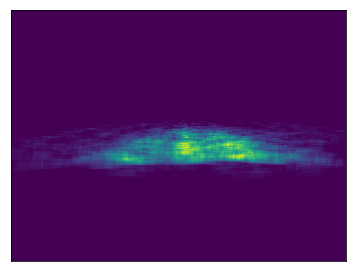
\includegraphics[width=0.8\linewidth]{images/pothole_locations_heatmap.png}
	\caption{Localizaciones de los socavones en las imágenes}
	\label{fig:potholeslocations}
\end{figure}

\subsection{Limpieza y normalización de los datos}

\textbf{!!! TODO}
\begin{itemize}
	\item explicar diferencia de tamaño entre redimensión directa vs crop + redimension
	\item explicar la normalización que se hace /255
	\item explicar el filtrado que se hace
\end{itemize} % (<4 páginas)

\newpage
\section{Técnicas de Deep Learning y métodos de evaluación}

% (<6 páginas)

\textbf{!!! TODO}

\subsection{Explicar las técnicas de DL que se van a utilizar en el proyecto}

% (Esto sería parte teórica)

\textbf{!!! TODO}

\subsection{Explicar los métodos de evaluación que se van a utilizar en el proyecto}

% (Esto sería parte teórica)

\textbf{!!! TODO} % (<6 páginas)

\newpage
\section{Implementación y evaluación de las técnicas}

% (Aquí no te pongo límite de páginas. Explícalo como quieras ya que es la parte en la que tienes que explicar el trabajo técnico que has realizado.)

\subsection{Detalles de la implementación de las técnicas de DL aplicadas}

% (Esto sería parte práctica)
% una especie de bitácora sin hablar en primera persona

\textbf{!!! TODO}

\subsection{Evaluación de las técnicas}

% (Esto sería parte práctica)

\textbf{!!! TODO} % ()Aquí no te pongo límite de páginas)

\newpage
\section{Resultados}

% (< 3 páginas)

\subsection{Resultados del proyecto}

\textbf{!!! TODO}
 % (< 3 páginas)

\newpage
\section{Conclusiones}

% (< 3  páginas)

\subsection{Evaluación del proyecto}

% explicar lo de yolo v3 tiny después de yolo v3
\textbf{!!! TODO}

\subsection{Alternativas y posibles mejoras que podrían haberse aplicado al proyecto (trabajos futuros)}

\textbf{!!! TODO}

\subsection{Conclusiones personales}

\textbf{!!! TODO} % (< 3  páginas)

\newpage
\printbibliography[title={Referencias}]

\end{document}
